\documentclass[11pt]{article}

% Packages
\usepackage{amsmath}
\usepackage{amssymb}
\usepackage{geometry}
\usepackage{graphicx}
\usepackage{pgfplots}
\usepackage{xcolor}
\usepackage{booktabs}
\usepackage{tcolorbox}

% Settings
\geometry{a4paper, margin=1in}
\pgfplotsset{compat=1.18}
\setlength{\parindent}{0pt}
\setlength{\parskip}{0.5em}

% Title Information
\title{\textbf{Homework 4.10: A Closer Look at Forced Mechanical Vibrations}}
\author{Tashfeen Omran}
\date{September 2026}

\begin{document}

\maketitle
\tableofcontents
\newpage

% ==========================================
% PART 1: Introduction, Context, and Prerequisites
% ==========================================
\section{Part 1: Comprehensive Introduction, Context, and Prerequisites}

\subsection{Core Concepts}
In the study of differential equations, one of the most profoundly practical applications is the modeling of mechanical vibrations. In previous sections, we explored \textit{free vibrations}, where a mass-spring system is set into motion and left alone. Now, we introduce an \textit{external forcing function}, $F(t)$, which continuously adds or removes energy from the system. 

Specifically, we focus on a sinusoidal forcing function, $F(t) = F_0 \cos(\gamma t)$, where $F_0$ is the amplitude of the force and $\gamma$ is the angular frequency of the force. The differential equation governing this system is:
\[ m y'' + b y' + k y = F_0 \cos(\gamma t) \]
where:
\begin{itemize}
    \item $m$ is the mass.
    \item $b$ is the damping constant (friction/air resistance).
    \item $k$ is the spring stiffness constant.
    \item $y(t)$ is the displacement from equilibrium at time $t$.
\end{itemize}

The general solution to this nonhomogeneous linear differential equation is the sum of two parts: $y(t) = y_h(t) + y_p(t)$.
\begin{itemize}
    \item \textbf{Transient Solution ($y_h(t)$):} The solution to the homogeneous equation ($m y'' + b y' + k y = 0$). If damping is present ($b > 0$), this term contains a decaying exponential ($e^{-\alpha t}$) and will eventually die out as $t \to \infty$.
    \item \textbf{Steady-State Solution ($y_p(t)$):} The particular solution driven by the external force. It does not die out. Once the transient solution fades, the system's motion is entirely dictated by $y_p(t)$.
\end{itemize}

\subsection{Intuition and Derivation}
Why does the system eventually synchronize with the external force? Imagine pushing a child on a swing. Initially, the swing's natural motion (transient) might clash with your pushes. But over time, the friction dampens the initial chaotic motion, and the swing moves exactly at the rhythm of your pushes (steady-state). 

Mathematically, we find $y_p(t)$ using the Method of Undetermined Coefficients. We guess a solution of the form $y_p(t) = A \cos(\gamma t) + B \sin(\gamma t)$. Substituting this into the differential equation and solving for $A$ and $B$ yields a combined sinusoidal wave:
\[ y_p(t) = \frac{F_0}{\sqrt{(k-m\gamma^2)^2 + b^2\gamma^2}} \sin(\gamma t + \theta) \]
The amplitude of this steady-state motion depends heavily on $\gamma$. The factor multiplying $F_0$ is called the \textbf{frequency gain}, $M(\gamma)$. When the forcing frequency $\gamma$ is close to the system's natural frequency, the denominator becomes very small, causing the amplitude to spike. This phenomenon is called \textbf{resonance}.

\subsection{Historical Context and Motivation}
The mathematical formalization of forced vibrations was driven by the industrial revolution and the advent of heavy machinery, bridges, and aircraft. Engineers noticed that machines would sometimes shake themselves to pieces even if the forces applied were relatively small. The most famous (though slightly nuanced) historical example is the collapse of the Tacoma Narrows Bridge in 1940, where wind provided a periodic forcing function that matched the bridge's natural frequency, leading to catastrophic oscillations. Understanding $M(\gamma)$ allows engineers to design systems with damping ($b$) and stiffness ($k$) that avoid resonance at expected operating frequencies.

\subsection{Key Formulas}
\begin{itemize}
    \item \textbf{Equation of Motion:} $m y'' + b y' + k y = F_{\text{ext}}(t)$
    \item \textbf{Frequency Gain:} $M(\gamma) = \frac{1}{\sqrt{(k-m\gamma^2)^2 + b^2\gamma^2}}$
    \item \textbf{Steady-State Amplitude:} $A_{\text{steady}} = F_0 \cdot M(\gamma)$
    \item \textbf{Phase Angle:} $\tan \theta = \frac{k-m\gamma^2}{b\gamma}$
    \item \textbf{Resonance Frequency (Damped):} $\gamma_r = \sqrt{\frac{k}{m} - \frac{b^2}{2m^2}}$ (Valid only if $b^2 < 2mk$)
    \item \textbf{Natural Frequency (Undamped):} $\omega = \sqrt{\frac{k}{m}}$
\end{itemize}

\subsection{Prerequisites}
To succeed in this topic, you must be proficient in:
1. Solving second-order linear homogeneous ODEs (finding roots of the characteristic equation).
2. The Method of Undetermined Coefficients.
3. Trigonometric identities (specifically sum-to-product formulas for analyzing "beats").
4. Converting between amplitude-phase form and standard sine/cosine sums: $A \cos(\omega t) + B \sin(\omega t) = R \sin(\omega t + \theta)$.
5. Basic calculus (differentiation to find velocity, setting derivatives to zero to find maximums).

\newpage
% ==========================================
% PART 2: Detailed Homework Solutions
% ==========================================
\section{Part 2: Detailed Homework Solutions}
\textit{Note on Strategic Selection: To maximize learning efficiency, I have selected a representative subset of problems (1, 2, 3, 4, 5, 8, 9, 11, 12, 13) that covers at least two of every distinct problem archetype found in this section (Curve Sketching, Undamped Resonance, Beats, Steady-State Word Problems, and Full IVP Word Problems).}

\subsection{Problem 1}
\textbf{Question:} Sketch the frequency response curve (13) for the system in which $m = 4$, $k = 1$, $b = 2$.

\textbf{Solution:}
The frequency response curve is given by the frequency gain function:
\[ M(\gamma) = \frac{1}{\sqrt{(k-m\gamma^2)^2 + b^2\gamma^2}} \]
Substitute the given values $m=4$, $k=1$, $b=2$:
\[ M(\gamma) = \frac{1}{\sqrt{(1-4\gamma^2)^2 + (2\gamma)^2}} = \frac{1}{\sqrt{(1-4\gamma^2)^2 + 4\gamma^2}} \]
To sketch this, we need to determine if there is a resonance peak. A peak occurs if $b^2 < 2mk$.
Let's check: $b^2 = 2^2 = 4$. $2mk = 2(4)(1) = 8$.
Since $4 < 8$, the system is underdamped enough to have a resonance peak.
The resonance frequency $\gamma_r$ is:
\[ \gamma_r = \sqrt{\frac{k}{m} - \frac{b^2}{2m^2}} = \sqrt{\frac{1}{4} - \frac{4}{2(16)}} = \sqrt{\frac{1}{4} - \frac{1}{8}} = \sqrt{\frac{1}{8}} = \frac{1}{2\sqrt{2}} \approx 0.354 \]
The maximum gain at resonance is:
\[ M(\gamma_r) = \frac{1}{\sqrt{(1-4(1/8))^2 + 4(1/8)}} = \frac{1}{\sqrt{(1-1/2)^2 + 1/2}} = \frac{1}{\sqrt{1/4 + 1/2}} = \frac{1}{\sqrt{3/4}} = \frac{2}{\sqrt{3}} \approx 1.155 \]
The $y$-intercept (when $\gamma = 0$) is:
\[ M(0) = \frac{1}{\sqrt{(1-0)^2 + 0}} = 1 \]
As $\gamma \to \infty$, $M(\gamma) \to 0$.

\begin{center}
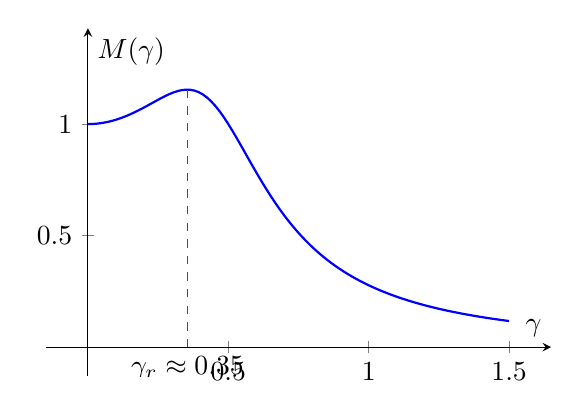
\begin{tikzpicture}
\begin{axis}[
    domain=0:1.5,
    samples=100,
    axis lines=middle,
    xlabel=$\gamma$,
    ylabel=$M(\gamma)$,
    enlargelimits=true,
    width=8cm,
    height=6cm,
    ymin=0, ymax=1.3
]
\addplot[thick, blue] {1/sqrt((1-4*x^2)^2 + 4*x^2)};
\addplot[dashed, red] coordinates {(0.354, 0) (0.354, 1.155)};
\node[below] at (axis cs:0.354,0) {$\gamma_r \approx 0.35$};
\end{axis}
\end{tikzpicture}
\end{center}

\subsection{Problem 2}
\textbf{Question:} Sketch the frequency response curve (13) for the system in which $m = 2$, $k = 3$, $b = 3$.

\textbf{Solution:}
Substitute $m=2$, $k=3$, $b=3$ into the gain function:
\[ M(\gamma) = \frac{1}{\sqrt{(3-2\gamma^2)^2 + (3\gamma)^2}} = \frac{1}{\sqrt{(3-2\gamma^2)^2 + 9\gamma^2}} \]
Check for a resonance peak ($b^2 < 2mk$):
$b^2 = 9$. $2mk = 2(2)(3) = 12$.
Since $9 < 12$, there is a resonance peak.
Find the resonance frequency $\gamma_r$:
\[ \gamma_r = \sqrt{\frac{k}{m} - \frac{b^2}{2m^2}} = \sqrt{\frac{3}{2} - \frac{9}{2(4)}} = \sqrt{\frac{12}{8} - \frac{9}{8}} = \sqrt{\frac{3}{8}} \approx 0.612 \]
The maximum gain at resonance is:
\[ M(\gamma_r) = \frac{1}{\sqrt{(3-2(3/8))^2 + 9(3/8)}} = \frac{1}{\sqrt{(3-3/4)^2 + 27/8}} = \frac{1}{\sqrt{(9/4)^2 + 27/8}} \]
\[ M(\gamma_r) = \frac{1}{\sqrt{81/16 + 54/16}} = \frac{1}{\sqrt{135/16}} = \frac{4}{\sqrt{135}} \approx 0.344 \]
The $y$-intercept (when $\gamma = 0$) is:
\[ M(0) = \frac{1}{\sqrt{(3-0)^2 + 0}} = \frac{1}{3} \approx 0.333 \]
Notice that the peak ($0.344$) is barely higher than the intercept ($0.333$). This is a highly damped system that is very close to the threshold of not having a peak at all.

\begin{center}
\begin{tikzpicture}
\begin{axis}[
    domain=0:2,
    samples=100,
    axis lines=middle,
    xlabel=$\gamma$,
    ylabel=$M(\gamma)$,
    enlargelimits=true,
    width=8cm,
    height=6cm,
    ymin=0, ymax=0.4
]
\addplot[thick, blue] {1/sqrt((3-2*x^2)^2 + 9*x^2)};
\addplot[dashed, red] coordinates {(0.612, 0) (0.612, 0.344)};
\end{axis}
\end{tikzpicture}
\end{center}

\subsection{Problem 3}
\textbf{Question:} Determine the equation of motion for an undamped system at resonance governed by:
\[ \frac{d^2y}{dt^2} + 9y = 2 \cos 3t \quad ; \quad y(0) = 1, \quad y'(0) = 0 \]

\textbf{Solution:}
\textbf{Step 1: Solve the homogeneous equation.}
\[ r^2 + 9 = 0 \implies r = \pm 3i \]
The complementary solution is:
\[ y_h(t) = c_1 \cos 3t + c_2 \sin 3t \]

\textbf{Step 2: Find the particular solution.}
The forcing function is $2 \cos 3t$. Normally, we would guess $y_p = A \cos 3t + B \sin 3t$. However, this overlaps with the homogeneous solution (this is the mathematical definition of resonance). Therefore, we must multiply our guess by $t$:
\[ y_p(t) = t(A \cos 3t + B \sin 3t) \]
Differentiate $y_p(t)$ using the product rule:
\[ y_p'(t) = (A \cos 3t + B \sin 3t) + t(-3A \sin 3t + 3B \cos 3t) \]
\[ y_p''(t) = (-3A \sin 3t + 3B \cos 3t) + (-3A \sin 3t + 3B \cos 3t) + t(-9A \cos 3t - 9B \sin 3t) \]
\[ y_p''(t) = -6A \sin 3t + 6B \cos 3t - 9t(A \cos 3t + B \sin 3t) \]
Substitute $y_p''$ and $y_p$ into the original ODE:
\[ [-6A \sin 3t + 6B \cos 3t - 9t(A \cos 3t + B \sin 3t)] + 9[t(A \cos 3t + B \sin 3t)] = 2 \cos 3t \]
The terms with $t$ cancel out perfectly:
\[ -6A \sin 3t + 6B \cos 3t = 2 \cos 3t \]
Equating coefficients:
\[ -6A = 0 \implies A = 0 \]
\[ 6B = 2 \implies B = \frac{1}{3} \]
Thus, $y_p(t) = \frac{1}{3} t \sin 3t$.

\textbf{Step 3: Apply initial conditions to the general solution.}
\[ y(t) = y_h(t) + y_p(t) = c_1 \cos 3t + c_2 \sin 3t + \frac{1}{3} t \sin 3t \]
Apply $y(0) = 1$:
\[ 1 = c_1(1) + c_2(0) + 0 \implies c_1 = 1 \]
Differentiate $y(t)$ to apply the second condition:
\[ y'(t) = -3c_1 \sin 3t + 3c_2 \cos 3t + \frac{1}{3} \sin 3t + t \cos 3t \]
Apply $y'(0) = 0$:
\[ 0 = -3(1)(0) + 3c_2(1) + 0 + 0 \implies 3c_2 = 0 \implies c_2 = 0 \]
\textbf{Final Answer:}
\[ y(t) = \cos 3t + \frac{1}{3} t \sin 3t \]

\subsection{Problem 4}
\textbf{Question:} Determine the equation of motion for an undamped system at resonance governed by:
\[ \frac{d^2y}{dt^2} + y = 5 \cos t \quad ; \quad y(0) = 0, \quad y'(0) = 1 \]

\textbf{Solution:}
\textbf{Step 1: Homogeneous solution.}
\[ r^2 + 1 = 0 \implies r = \pm i \]
\[ y_h(t) = c_1 \cos t + c_2 \sin t \]

\textbf{Step 2: Particular solution.}
Because the forcing frequency ($\gamma = 1$) matches the natural frequency ($\omega = 1$), we guess:
\[ y_p(t) = t(A \cos t + B \sin t) \]
\[ y_p'(t) = (A \cos t + B \sin t) + t(-A \sin t + B \cos t) \]
\[ y_p''(t) = -2A \sin t + 2B \cos t - t(A \cos t + B \sin t) \]
Substitute into $y'' + y = 5 \cos t$:
\[ [-2A \sin t + 2B \cos t - t(A \cos t + B \sin t)] + t(A \cos t + B \sin t) = 5 \cos t \]
\[ -2A \sin t + 2B \cos t = 5 \cos t \]
Equating coefficients:
\[ -2A = 0 \implies A = 0 \]
\[ 2B = 5 \implies B = \frac{5}{2} \]
Thus, $y_p(t) = \frac{5}{2} t \sin t$.

\textbf{Step 3: Apply initial conditions.}
\[ y(t) = c_1 \cos t + c_2 \sin t + \frac{5}{2} t \sin t \]
Apply $y(0) = 0$:
\[ 0 = c_1(1) + 0 + 0 \implies c_1 = 0 \]
Differentiate $y(t)$:
\[ y'(t) = c_2 \cos t + \frac{5}{2} \sin t + \frac{5}{2} t \cos t \]
Apply $y'(0) = 1$:
\[ 1 = c_2(1) + 0 + 0 \implies c_2 = 1 \]
\textbf{Final Answer:}
\[ y(t) = \sin t + \frac{5}{2} t \sin t \]

\subsection{Problem 5}
\textbf{Question:} An undamped system is governed by $m \frac{d^2y}{dt^2} + ky = F_0 \cos \gamma t ; y(0)=y'(0)=0$, where $\gamma \neq \omega = \sqrt{k/m}$.
(a) Find the equation of motion.
(b) Use trigonometric identities to show the solution can be written as $y(t) = \frac{2F_0}{m(\omega^2 - \gamma^2)} \sin\left(\frac{\omega+\gamma}{2}t\right) \sin\left(\frac{\omega-\gamma}{2}t\right)$.

\textbf{Solution:}
\textbf{Part (a):}
The homogeneous solution is $y_h(t) = c_1 \cos \omega t + c_2 \sin \omega t$.
Since $\gamma \neq \omega$, we guess $y_p(t) = A \cos \gamma t$.
Substitute into the ODE:
\[ m(-\gamma^2 A \cos \gamma t) + k(A \cos \gamma t) = F_0 \cos \gamma t \]
\[ A(k - m\gamma^2) = F_0 \implies A = \frac{F_0}{k - m\gamma^2} \]
Since $\omega^2 = k/m$, we can write $k = m\omega^2$. Thus, $A = \frac{F_0}{m(\omega^2 - \gamma^2)}$.
The general solution is:
\[ y(t) = c_1 \cos \omega t + c_2 \sin \omega t + \frac{F_0}{m(\omega^2 - \gamma^2)} \cos \gamma t \]
Apply $y(0) = 0$:
\[ 0 = c_1 + \frac{F_0}{m(\omega^2 - \gamma^2)} \implies c_1 = -\frac{F_0}{m(\omega^2 - \gamma^2)} \]
Apply $y'(0) = 0$:
\[ y'(t) = -c_1 \omega \sin \omega t + c_2 \omega \cos \omega t - \frac{F_0 \gamma}{m(\omega^2 - \gamma^2)} \sin \gamma t \]
\[ 0 = c_2 \omega \implies c_2 = 0 \]
\textbf{Answer (a):}
\[ y(t) = \frac{F_0}{m(\omega^2 - \gamma^2)} (\cos \gamma t - \cos \omega t) \]

\textbf{Part (b):}
We use the sum-to-product trigonometric identity:
\[ \cos A - \cos B = -2 \sin\left(\frac{A+B}{2}\right) \sin\left(\frac{A-B}{2}\right) \]
Let $A = \gamma t$ and $B = \omega t$:
\[ \cos \gamma t - \cos \omega t = -2 \sin\left(\frac{\gamma + \omega}{2}t\right) \sin\left(\frac{\gamma - \omega}{2}t\right) \]
Because sine is an odd function ($\sin(-x) = -\sin(x)$), we can absorb the negative sign into the second sine term:
\[ -2 \sin\left(\frac{\gamma + \omega}{2}t\right) \sin\left(-\frac{\omega - \gamma}{2}t\right) = 2 \sin\left(\frac{\omega + \gamma}{2}t\right) \sin\left(\frac{\omega - \gamma}{2}t\right) \]
Substitute this back into our equation of motion:
\textbf{Answer (b):}
\[ y(t) = \frac{2F_0}{m(\omega^2 - \gamma^2)} \sin\left(\frac{\omega + \gamma}{2}t\right) \sin\left(\frac{\omega - \gamma}{2}t\right) \]
\textit{This form clearly shows the phenomenon of "beats"—a high-frequency oscillation modulated by a low-frequency envelope.}

\subsection{Problem 8}
\textbf{Question:} The response of an overdamped system to a constant force is governed by $2y'' + 8y' + 6y = 18$, with $y(0)=0, y'(0)=0$. Compute and sketch the displacement $y(t)$. What is the limiting value of $y(t)$ as $t \to \infty$? Interpret physically.

\textbf{Solution:}
\textbf{Step 1: Homogeneous solution.}
\[ 2r^2 + 8r + 6 = 0 \implies r^2 + 4r + 3 = 0 \implies (r+1)(r+3) = 0 \]
Roots are $r = -1, -3$.
\[ y_h(t) = c_1 e^{-t} + c_2 e^{-3t} \]

\textbf{Step 2: Particular solution.}
The forcing function is a constant ($18$). Guess $y_p(t) = A$.
Substitute into ODE: $2(0) + 8(0) + 6A = 18 \implies A = 3$.
\[ y(t) = c_1 e^{-t} + c_2 e^{-3t} + 3 \]

\textbf{Step 3: Initial conditions.}
\[ y(0) = c_1 + c_2 + 3 = 0 \implies c_1 + c_2 = -3 \]
\[ y'(t) = -c_1 e^{-t} - 3c_2 e^{-3t} \]
\[ y'(0) = -c_1 - 3c_2 = 0 \implies c_1 = -3c_2 \]
Substitute $c_1$ into the first equation:
\[ -3c_2 + c_2 = -3 \implies -2c_2 = -3 \implies c_2 = 1.5 \]
\[ c_1 = -3(1.5) = -4.5 \]
\textbf{Equation of Motion:}
\[ y(t) = -4.5 e^{-t} + 1.5 e^{-3t} + 3 \]

\textbf{Limiting Value:}
\[ \lim_{t \to \infty} y(t) = \lim_{t \to \infty} (-4.5 e^{-t} + 1.5 e^{-3t} + 3) = 0 + 0 + 3 = 3 \]
\textbf{Physical Interpretation:} The constant external force of $18$ N shifts the equilibrium position of the spring by $3$ meters. Because the system is overdamped, it smoothly approaches this new equilibrium position without oscillating.

\subsection{Problem 9}
\textbf{Question:} An 8-kg mass is attached to a spring, stretching it 1.96 m to equilibrium. At $t=0$, an external force $F(t) = \cos 2t$ N is applied. Damping constant is 3 N-sec/m. Determine the steady-state solution.

\textbf{Solution:}
\textbf{Step 1: Find system parameters.}
Mass $m = 8$ kg.
Spring constant $k$: At equilibrium, $mg = kL \implies k = \frac{mg}{L} = \frac{8 \times 9.8}{1.96} = \frac{78.4}{1.96} = 40$ N/m.
Damping $b = 3$.
Forcing function $F(t) = 1 \cos 2t \implies F_0 = 1, \gamma = 2$.

\textbf{Step 2: Use the steady-state formula.}
The steady-state solution is $y_p(t) = \frac{F_0}{\sqrt{(k-m\gamma^2)^2 + b^2\gamma^2}} \sin(\gamma t + \theta)$.
Calculate the components:
\[ k - m\gamma^2 = 40 - 8(2^2) = 40 - 32 = 8 \]
\[ b\gamma = 3(2) = 6 \]
Denominator: $\sqrt{8^2 + 6^2} = \sqrt{64 + 36} = \sqrt{100} = 10$.
Amplitude: $\frac{F_0}{10} = \frac{1}{10} = 0.1$.

Calculate the phase angle $\theta$:
\[ \tan \theta = \frac{k-m\gamma^2}{b\gamma} = \frac{8}{6} = \frac{4}{3} \]
Since both the numerator and denominator are positive, $\theta$ is in Quadrant I.
\[ \theta = \arctan\left(\frac{4}{3}\right) \approx 0.927 \text{ radians} \]
\textbf{Final Answer:}
\[ y_p(t) = 0.1 \sin(2t + 0.927) \]

\subsection{Problem 11}
\textbf{Question:} An 8-lb weight is attached to a spring, stretching it 20 cm (Wait, the text says "A mass weighing 8 lb is attached... If the spring constant is 10 lb/ft and damping is 1 lb-sec/ft... $F(t) = 2\cos 2t$"). Find the equation of motion. What is the resonance frequency?

\textbf{Solution:}
\textbf{Step 1: Find system parameters.}
Weight $W = 8$ lb. Mass $m = \frac{W}{g} = \frac{8}{32} = \frac{1}{4}$ slugs.
Spring constant $k = 10$ lb/ft.
Damping $b = 1$ lb-sec/ft.
Forcing function $F(t) = 2 \cos 2t \implies F_0 = 2, \gamma = 2$.
Initial conditions: "comes to rest at its equilibrium position" means $y(0) = 0, y'(0) = 0$.
ODE: $\frac{1}{4}y'' + y' + 10y = 2 \cos 2t \implies y'' + 4y' + 40y = 8 \cos 2t$.

\textbf{Step 2: Homogeneous solution.}
\[ r^2 + 4r + 40 = 0 \implies r = \frac{-4 \pm \sqrt{16 - 160}}{2} = \frac{-4 \pm \sqrt{-144}}{2} = -2 \pm 6i \]
\[ y_h(t) = e^{-2t}(c_1 \cos 6t + c_2 \sin 6t) \]

\textbf{Step 3: Particular solution.}
Guess $y_p(t) = A \cos 2t + B \sin 2t$.
\[ y_p' = -2A \sin 2t + 2B \cos 2t \]
\[ y_p'' = -4A \cos 2t - 4B \sin 2t \]
Substitute into $y'' + 4y' + 40y = 8 \cos 2t$:
\[ (-4A \cos 2t - 4B \sin 2t) + 4(-2A \sin 2t + 2B \cos 2t) + 40(A \cos 2t + B \sin 2t) = 8 \cos 2t \]
Group cosines: $-4A + 8B + 40A = 8 \implies 36A + 8B = 8 \implies 9A + 2B = 2$.
Group sines: $-4B - 8A + 40B = 0 \implies -8A + 36B = 0 \implies 2A = 9B \implies A = 4.5B$.
Substitute $A$ into the first equation:
\[ 9(4.5B) + 2B = 2 \implies 40.5B + 2B = 2 \implies 42.5B = 2 \implies B = \frac{2}{42.5} = \frac{4}{85} \]
\[ A = 4.5 \left(\frac{4}{85}\right) = \frac{18}{85} \]
\[ y_p(t) = \frac{18}{85} \cos 2t + \frac{4}{85} \sin 2t \]

\textbf{Step 4: Apply initial conditions.}
\[ y(t) = e^{-2t}(c_1 \cos 6t + c_2 \sin 6t) + \frac{18}{85} \cos 2t + \frac{4}{85} \sin 2t \]
\[ y(0) = c_1 + \frac{18}{85} = 0 \implies c_1 = -\frac{18}{85} \]
Differentiate $y(t)$:
\[ y'(t) = -2e^{-2t}(c_1 \cos 6t + c_2 \sin 6t) + e^{-2t}(-6c_1 \sin 6t + 6c_2 \cos 6t) - \frac{36}{85} \sin 2t + \frac{8}{85} \cos 2t \]
\[ y'(0) = -2c_1 + 6c_2 + \frac{8}{85} = 0 \]
Substitute $c_1$:
\[ -2\left(-\frac{18}{85}\right) + 6c_2 + \frac{8}{85} = 0 \implies \frac{36}{85} + \frac{8}{85} + 6c_2 = 0 \implies \frac{44}{85} + 6c_2 = 0 \]
\[ 6c_2 = -\frac{44}{85} \implies c_2 = -\frac{44}{510} = -\frac{22}{255} \]
\textbf{Equation of Motion:}
\[ y(t) = e^{-2t}\left(-\frac{18}{85} \cos 6t - \frac{22}{255} \sin 6t\right) + \frac{18}{85} \cos 2t + \frac{4}{85} \sin 2t \]

\textbf{Step 5: Resonance Frequency.}
\[ \gamma_r = \sqrt{\frac{k}{m} - \frac{b^2}{2m^2}} = \sqrt{\frac{10}{1/4} - \frac{1^2}{2(1/16)}} = \sqrt{40 - \frac{1}{1/8}} = \sqrt{40 - 8} = \sqrt{32} = 4\sqrt{2} \text{ rad/sec} \]
In Hertz: $f_r = \frac{\gamma_r}{2\pi} = \frac{4\sqrt{2}}{2\pi} = \frac{2\sqrt{2}}{\pi}$ Hz.

\subsection{Problem 12}
\textbf{Question:} A 2-kg mass stretches a spring 20 cm. At $t=0$, mass is displaced 5 cm below equilibrium and released. $F(t) = 0.3 \cos t$ is applied. Damping is 5 N-sec/m. Find equation of motion and resonance frequency.

\textbf{Solution:}
\textbf{Step 1: Parameters.}
$m = 2$ kg.
$L = 20$ cm $= 0.2$ m. $k = \frac{mg}{L} = \frac{2(9.8)}{0.2} = 98$ N/m.
$b = 5$.
$F(t) = 0.3 \cos t \implies F_0 = 0.3, \gamma = 1$.
Initial conditions: $y(0) = 0.05$ m, $y'(0) = 0$.
ODE: $2y'' + 5y' + 98y = 0.3 \cos t$.

\textbf{Step 2: Homogeneous solution.}
\[ 2r^2 + 5r + 98 = 0 \implies r = \frac{-5 \pm \sqrt{25 - 4(2)(98)}}{4} = \frac{-5 \pm \sqrt{25 - 784}}{4} = -1.25 \pm \frac{\sqrt{759}}{4}i \]
Let $\omega_d = \frac{\sqrt{759}}{4} \approx 6.887$.
\[ y_h(t) = e^{-1.25t}(c_1 \cos \omega_d t + c_2 \sin \omega_d t) \]

\textbf{Step 3: Particular solution.}
Guess $y_p = A \cos t + B \sin t$.
Substitute into ODE:
\[ 2(-A \cos t - B \sin t) + 5(-A \sin t + B \cos t) + 98(A \cos t + B \sin t) = 0.3 \cos t \]
Cosines: $-2A + 5B + 98A = 0.3 \implies 96A + 5B = 0.3$.
Sines: $-2B - 5A + 98B = 0 \implies -5A + 96B = 0 \implies A = 19.2B$.
Substitute $A$:
\[ 96(19.2B) + 5B = 0.3 \implies 1843.2B + 5B = 0.3 \implies 1848.2B = 0.3 \implies B \approx 0.000162 \]
\[ A = 19.2(0.000162) \approx 0.003116 \]
\[ y_p(t) = 0.003116 \cos t + 0.000162 \sin t \]

\textbf{Step 4: Initial conditions.}
\[ y(0) = c_1 + A = 0.05 \implies c_1 = 0.05 - 0.003116 = 0.046884 \]
\[ y'(0) = -1.25c_1 + \omega_d c_2 + B = 0 \implies c_2 = \frac{1.25c_1 - B}{\omega_d} \]
\[ c_2 = \frac{1.25(0.046884) - 0.000162}{6.887} \approx \frac{0.058605 - 0.000162}{6.887} \approx 0.008486 \]
\textbf{Equation of Motion:}
\[ y(t) \approx e^{-1.25t}(0.0469 \cos 6.887t + 0.0085 \sin 6.887t) + 0.0031 \cos t + 0.0002 \sin t \]

\textbf{Step 5: Resonance Frequency.}
\[ \gamma_r = \sqrt{\frac{k}{m} - \frac{b^2}{2m^2}} = \sqrt{\frac{98}{2} - \frac{25}{2(4)}} = \sqrt{49 - 3.125} = \sqrt{45.875} \approx 6.773 \text{ rad/sec} \]
In Hertz: $f_r = \frac{6.773}{2\pi} \approx 1.078$ Hz.

\subsection{Problem 13}
\textbf{Question:} A 32-lb weight is attached to a spring. $k = 5$ lb/ft, $b = 2$ lb-sec/ft. $F(t) = 3 \cos 4t$. Find the steady-state solution.

\textbf{Solution:}
$m = \frac{32}{32} = 1$ slug. $k = 5$, $b = 2$, $F_0 = 3$, $\gamma = 4$.
Steady-state formula: $y_p(t) = \frac{F_0}{\sqrt{(k-m\gamma^2)^2 + b^2\gamma^2}} \sin(\gamma t + \theta)$.
\[ k - m\gamma^2 = 5 - 1(4^2) = 5 - 16 = -11 \]
\[ b\gamma = 2(4) = 8 \]
Denominator: $\sqrt{(-11)^2 + 8^2} = \sqrt{121 + 64} = \sqrt{185}$.
Amplitude: $\frac{3}{\sqrt{185}}$.
Phase angle: $\tan \theta = \frac{-11}{8}$.
Since the numerator is negative and the denominator is positive, $\theta$ is in Quadrant IV.
\[ \theta = \arctan\left(-\frac{11}{8}\right) \approx -0.942 \text{ radians} \]
\textbf{Final Answer:}
\[ y_p(t) = \frac{3}{\sqrt{185}} \sin(4t - 0.942) \]

\newpage
% ==========================================
% PART 3: In-Depth Analysis of Problems and Techniques
% ==========================================
\section{Part 3: In-Depth Analysis of Problems and Techniques}

\subsection{A) Problem Types and General Approach}
The homework problems fall into several distinct archetypes, each requiring a specific strategy:

\begin{enumerate}
    \item \textbf{Frequency Response Curve Sketching (Problems 1, 2):}
    \textit{Strategy:} Plug the system parameters into the $M(\gamma)$ formula. Calculate the limits as $\gamma \to 0$ and $\gamma \to \infty$. Crucially, check the discriminant $b^2 < 2mk$ to see if a resonance peak exists. If it does, calculate $\gamma_r$ and $M(\gamma_r)$ to plot the maximum point.
    
    \item \textbf{Undamped Resonance (Problems 3, 4):}
    \textit{Strategy:} Recognize that $b=0$ and the forcing frequency $\gamma$ exactly matches the natural frequency $\omega = \sqrt{k/m}$. Because of this overlap, the standard guess for Undetermined Coefficients fails. You must multiply the guess by $t$: $y_p(t) = t(A \cos \gamma t + B \sin \gamma t)$.
    
    \item \textbf{Steady-State Extraction (Problems 9, 13):}
    \textit{Strategy:} These problems do not ask for the full equation of motion, saving you from solving for $c_1$ and $c_2$. Instead, directly apply the amplitude-phase formula for $y_p(t)$. The most critical step is correctly identifying the quadrant for the phase angle $\theta$ based on the signs of the numerator and denominator of $\tan \theta$.
    
    \item \textbf{Full Initial Value Problems (Problems 11, 12):}
    \textit{Strategy:} This is the most labor-intensive type. You must find $y_h(t)$, find $y_p(t)$ using Undetermined Coefficients, combine them into $y(t) = y_h(t) + y_p(t)$, and \textit{only then} apply the initial conditions $y(0)$ and $y'(0)$. A common trap is applying initial conditions to $y_h(t)$ before adding $y_p(t)$.
    
    \item \textbf{Theoretical / Beats (Problem 5):}
    \textit{Strategy:} These require algebraic manipulation rather than numerical calculation. The key is using trigonometric sum-to-product identities to transform a sum of cosines into a product of sines, revealing the "envelope" structure of the beats phenomenon.
\end{enumerate}

\subsection{B) Key Algebraic and Calculus Manipulations}
\begin{itemize}
    \item \textbf{The "$t$-Multiplier" Trick (Calculus):} Used in Problems 3 and 4. When the forcing function is a solution to the homogeneous equation, the standard particular solution guess yields $0 = F(t)$. Multiplying by $t$ introduces product-rule derivatives that perfectly cancel the homogeneous parts, leaving behind solvable algebraic terms.
    \item \textbf{Sum-to-Product Identities (Algebra/Trig):} Used in Problem 5. The identity $\cos A - \cos B = -2 \sin(\frac{A+B}{2}) \sin(\frac{A-B}{2})$ is essential for proving that two superimposed waves of slightly different frequencies create a single wave with a slowly varying amplitude (beats).
    \item \textbf{Quadrant Checking for Phase Angle (Trig):} Used in Problems 9 and 13. The formula $\tan \theta = \frac{k-m\gamma^2}{b\gamma}$ is dangerous if plugged blindly into a calculator's $\arctan$ function, which only returns values in Quadrants I and IV. You must manually check the signs: if the numerator is positive and denominator positive $\to$ Quad I. If numerator negative and denominator positive $\to$ Quad IV.
    \item \textbf{Unit Conversion (Algebra/Physics):} Used in Problems 11 and 13. In the US Customary System, weight (lbs) is a force, not a mass. You must divide by gravity ($g = 32$ ft/sec$^2$) to find the mass in slugs before setting up the differential equation.
\end{itemize}

\newpage
% ==========================================
% PART 4: "Cheatsheet" and Tips for Success
% ==========================================
\section{Part 4: "Cheatsheet" and Tips for Success}

\begin{tcolorbox}[colback=blue!5,colframe=blue!40!black,title=Essential Formulas]
\textbf{Standard Form:} $m y'' + b y' + k y = F_0 \cos(\gamma t)$ \\
\textbf{Natural Frequency (Undamped):} $\omega = \sqrt{\frac{k}{m}}$ \\
\textbf{Resonance Frequency (Damped):} $\gamma_r = \sqrt{\frac{k}{m} - \frac{b^2}{2m^2}}$ \quad (Requires $b^2 < 2mk$) \\
\textbf{Steady-State Solution:} $y_p(t) = \frac{F_0}{\sqrt{(k-m\gamma^2)^2 + b^2\gamma^2}} \sin(\gamma t + \theta)$ \\
\textbf{Phase Angle:} $\tan \theta = \frac{k-m\gamma^2}{b\gamma}$
\end{tcolorbox}

\subsection{Shortcuts and Tricks}
\begin{itemize}
    \item \textbf{Bypass Undetermined Coefficients for Steady-State:} If a question \textit{only} asks for the steady-state solution, do not waste 10 minutes setting up $y_p = A \cos \gamma t + B \sin \gamma t$ and solving the massive system of equations. Jump straight to the amplitude-phase formula in the cheatsheet above.
    \item \textbf{Quick Resonance Check:} Before calculating $\gamma_r$, quickly check $b^2 < 2mk$. If $b^2 \geq 2mk$, the system is too damped to resonate, and the maximum amplitude occurs at $\gamma = 0$.
\end{itemize}

\subsection{Common Pitfalls and Traps}
\begin{itemize}
    \item \textbf{The Initial Condition Trap:} Never apply $y(0)$ and $y'(0)$ to the homogeneous solution $y_h(t)$ alone. Initial conditions apply to the \textit{entire} system $y(t) = y_h(t) + y_p(t)$.
    \item \textbf{The Mass vs. Weight Trap:} If a problem says "A 10-lb weight...", $m \neq 10$. $m = 10/32$. If a problem says "A 10-kg mass...", $m = 10$. Pay strict attention to units.
    \item \textbf{The Spring Constant Trap:} Sometimes $k$ is not given directly. If a mass stretches a spring by length $L$ to reach equilibrium, use Hooke's Law: $mg = kL \implies k = mg/L$. Make sure $L$ is in meters or feet, not centimeters or inches!
\end{itemize}

\newpage
% ==========================================
% PART 5: Conceptual Synthesis and The "Big Picture"
% ==========================================
\section{Part 5: Conceptual Synthesis and The "Big Picture"}

\subsection{A) Thematic Connections}
The core theme of this topic is \textbf{System Response to Stimulus in the Frequency Domain}. Throughout calculus, we usually think in the "time domain"—how things change second by second. Forced vibrations force us to think in the "frequency domain"—how a system's behavior changes based on the \textit{speed} of the input, rather than just the time. 

This theme appears in earlier calculus when we studied Taylor Series (approximating complex functions with polynomials of varying "frequencies" of curvature) and will appear heavily in Linear Algebra (eigenvalues representing natural frequencies of multi-dimensional systems).

\subsection{B) Forward and Backward Links}
\textbf{Backward Links:} This topic is the ultimate culmination of everything learned in basic differential equations. It requires the characteristic equation (from homogeneous ODEs), the Method of Undetermined Coefficients (from nonhomogeneous ODEs), and basic Newtonian physics.

\textbf{Forward Links:} Understanding $M(\gamma)$ (Frequency Gain) is the absolute bedrock for \textbf{Control Theory} and \textbf{Signal Processing}. In later engineering and math courses, you will learn the Laplace Transform. The messy algebraic fraction we used for amplitude, $\frac{1}{\sqrt{(k-m\gamma^2)^2 + b^2\gamma^2}}$, is actually the magnitude of the system's \textit{Transfer Function} evaluated along the imaginary axis in the complex plane ($s = i\gamma$). Mastering this now makes advanced topics like Bode Plots and Fourier Transforms highly intuitive.

\newpage
% ==========================================
% PART 6: Abstract Real-World Modeling
% ==========================================
\section{Part 6: Abstract Real-World Modeling (AI, ML, \& Quant Finance)}

\subsection{A) Concrete Scenarios}
While springs and masses are physical, the differential equation $my'' + by' + ky = F(t)$ models any system with inertia ($m$), friction/decay ($b$), mean-reversion ($k$), and external shocks ($F$).
\begin{enumerate}
    \item \textbf{Machine Learning (Gradient Descent with Momentum):} In training deep neural networks, standard gradient descent can get stuck. Adding "momentum" simulates a mass rolling down the loss landscape. The learning rate acts as the inverse of damping. If the data batches have a periodic bias (a forcing function), the optimizer can experience "resonance," causing the loss to wildly oscillate and diverge.
    \item \textbf{Quantitative Finance (Business Cycle Modeling):} Asset prices often exhibit mean-reversion (a "spring" pulling the price back to its fundamental value) and momentum (inertia). Central bank interest rate cycles act as a periodic forcing function.
\end{enumerate}

\subsection{B) Model Problem Setup: Stochastic Mean-Reversion with Periodic Drift}
Let's build a rigorous mathematical model for the Quantitative Finance scenario using Stochastic Calculus.

\textbf{State Space and Variables:}
Let $X_t$ be the spread between two cointegrated assets (e.g., two oil companies) at time $t$.
Let $\mu$ be the long-term equilibrium spread.
Let $\kappa$ be the speed of mean reversion (analogous to spring stiffness $k$).
Let $\sigma$ be the volatility of the spread.
Let $W_t$ be a standard Brownian motion under the risk-neutral probability measure $\mathbb{Q}$.

\textbf{The Forcing Function:}
Suppose macroeconomic seasonality (e.g., winter heating demand) applies a periodic deterministic force to the spread, modeled as $A \cos(\gamma t)$.

\textbf{The Stochastic Differential Equation (SDE):}
We model this using a modified Ornstein-Uhlenbeck (OU) process. The standard OU process is $dX_t = \kappa(\mu - X_t)dt + \sigma dW_t$. We inject our forcing function into the drift term:
\[ dX_t = \left[ \kappa(\mu - X_t) + A \cos(\gamma t) \right] dt + \sigma dW_t \]

\textbf{Solving via Ito's Lemma:}
To find the expected value of the spread $\mathbb{E}[X_t]$, we apply an integrating factor $e^{\kappa t}$. Let $Y_t = X_t e^{\kappa t}$. By Ito's Lemma:
\[ dY_t = \kappa X_t e^{\kappa t} dt + e^{\kappa t} dX_t \]
Substitute $dX_t$:
\[ dY_t = \kappa X_t e^{\kappa t} dt + e^{\kappa t} \left[ (\kappa\mu - \kappa X_t + A \cos(\gamma t)) dt + \sigma dW_t \right] \]
\[ dY_t = e^{\kappa t} (\kappa\mu + A \cos(\gamma t)) dt + \sigma e^{\kappa t} dW_t \]
Integrating from $0$ to $t$:
\[ X_t e^{\kappa t} = X_0 + \int_0^t e^{\kappa s} (\kappa\mu + A \cos(\gamma s)) ds + \int_0^t \sigma e^{\kappa s} dW_s \]
Taking the expectation $\mathbb{E}[\cdot]$ eliminates the Ito integral (since it's a martingale):
\[ \mathbb{E}[X_t] = X_0 e^{-\kappa t} + \mu(1 - e^{-\kappa t}) + A e^{-\kappa t} \int_0^t e^{\kappa s} \cos(\gamma s) ds \]
The integral $\int e^{\kappa s} \cos(\gamma s) ds$ is solved via integration by parts, yielding a steady-state sinusoidal response exactly analogous to the mechanical $y_p(t)$, showing how the financial spread will permanently oscillate around $\mu$ due to the seasonal forcing function.

\newpage
% ==========================================
% PART 7: Common Variations and Untested Concepts
% ==========================================
\section{Part 7: Common Variations and Untested Concepts}

Based on standard differential equations curricula, there is a highly powerful technique for solving forced vibrations that was \textit{not} required in this specific homework set: \textbf{The Complex Exponential Method}.

\subsection{The Complex Exponential Method}
Instead of guessing $y_p = A \cos \gamma t + B \sin \gamma t$ and solving a $2 \times 2$ system of equations, we can use Euler's Formula: $e^{i\gamma t} = \cos \gamma t + i \sin \gamma t$. 

If the forcing function is $F_0 \cos \gamma t$, we can replace it with $F_0 e^{i\gamma t}$, solve the differential equation in the complex plane, and then simply take the \textit{real part} of the answer at the end.

\textbf{Worked Example:}
Find the steady-state solution for $y'' + 2y' + 5y = 10 \cos t$.

\textit{Standard way:} Guess $A \cos t + B \sin t$, differentiate twice, group terms, solve for $A$ and $B$. (Tedious).

\textit{Complex way:}
Consider the complex ODE: $z'' + 2z' + 5z = 10 e^{it}$.
Guess $z_p(t) = C e^{it}$, where $C$ is a complex constant.
Differentiate: $z_p' = iC e^{it}$, $z_p'' = -C e^{it}$.
Substitute into the ODE:
\[ -C e^{it} + 2iC e^{it} + 5C e^{it} = 10 e^{it} \]
Divide by $e^{it}$:
\[ C(-1 + 2i + 5) = 10 \implies C(4 + 2i) = 10 \]
Solve for $C$:
\[ C = \frac{10}{4 + 2i} = \frac{10(4 - 2i)}{(4 + 2i)(4 - 2i)} = \frac{40 - 20i}{16 + 4} = \frac{40 - 20i}{20} = 2 - i \]
So the complex solution is:
\[ z_p(t) = (2 - i) e^{it} = (2 - i)(\cos t + i \sin t) \]
Expand this:
\[ z_p(t) = 2 \cos t + 2i \sin t - i \cos t - i^2 \sin t = (2 \cos t + \sin t) + i(2 \sin t - \cos t) \]
Since our original forcing function was $10 \cos t$ (the real part of $10 e^{it}$), our steady-state solution is simply the real part of $z_p(t)$:
\[ y_p(t) = \text{Re}(z_p(t)) = 2 \cos t + \sin t \]
This method completely bypasses the need to solve systems of equations and is heavily used in electrical engineering (phasor analysis).

\newpage
% ==========================================
% PART 8: Advanced Diagnostic Testing: "Find the Flaw"
% ==========================================
\section{Part 8: Advanced Diagnostic Testing: "Find the Flaw"}

Below are five problems with complete solutions. However, each solution contains a single, subtle, yet critical flaw. Your task as the grader is to find the error, explain why it is wrong in one sentence, and provide the correct final answer.

\subsection{Problem 1: Undamped Resonance}
\textbf{Problem:} Find the general solution to $y'' + 16y = 3 \cos 4t$.
\textbf{Flawed Solution:}
1. Homogeneous: $r^2 + 16 = 0 \implies r = \pm 4i$. So $y_h = c_1 \cos 4t + c_2 \sin 4t$.
2. Particular: Guess $y_p = A \cos 4t + B \sin 4t$.
3. Differentiate: $y_p'' = -16A \cos 4t - 16B \sin 4t$.
4. Substitute: $(-16A \cos 4t - 16B \sin 4t) + 16(A \cos 4t + B \sin 4t) = 3 \cos 4t$.
5. Simplify: $0 = 3 \cos 4t$.
6. Conclusion: Because $0 \neq 3 \cos 4t$, there is no particular solution to this differential equation.

\subsection{Problem 2: US Customary Units}
\textbf{Problem:} A 16-lb weight is attached to a spring with $k=2$ lb/ft. Damping is $b=1$. Find the resonance frequency $\gamma_r$.
\textbf{Flawed Solution:}
1. Identify parameters: $m = 16$, $k = 2$, $b = 1$.
2. Formula: $\gamma_r = \sqrt{\frac{k}{m} - \frac{b^2}{2m^2}}$.
3. Substitute: $\gamma_r = \sqrt{\frac{2}{16} - \frac{1}{2(256)}} = \sqrt{\frac{1}{8} - \frac{1}{512}} = \sqrt{\frac{64}{512} - \frac{1}{512}} = \sqrt{\frac{63}{512}}$.
4. Final Answer: $\gamma_r \approx 0.35$ rad/sec.

\subsection{Problem 3: Resonance Frequency Definition}
\textbf{Problem:} Find the resonance frequency for the system $y'' + 2y' + 10y = \cos \gamma t$.
\textbf{Flawed Solution:}
1. Identify parameters: $m = 1$, $b = 2$, $k = 10$.
2. Resonance occurs when the forcing frequency matches the natural frequency of the system.
3. Natural frequency $\omega = \sqrt{\frac{k}{m}} = \sqrt{\frac{10}{1}} = \sqrt{10}$.
4. Final Answer: The resonance frequency is $\sqrt{10}$ rad/sec.

\subsection{Problem 4: Phase Angle Quadrant}
\textbf{Problem:} Find the phase angle $\theta$ for the steady-state solution of $y'' + 3y' + 2y = \cos 3t$.
\textbf{Flawed Solution:}
1. Parameters: $m=1, b=3, k=2, \gamma=3$.
2. Formula: $\tan \theta = \frac{k-m\gamma^2}{b\gamma}$.
3. Substitute: $\tan \theta = \frac{2 - 1(9)}{3(3)} = \frac{-7}{9}$.
4. Calculate: $\theta = \arctan(-7/9) \approx -0.66$ radians.
5. Because the tangent is negative, we must add $\pi$ to find the true angle.
6. Final Answer: $\theta = -0.66 + \pi = 2.48$ radians (Quadrant II).

\subsection{Problem 5: Amplitude Calculation}
\textbf{Problem:} Find the amplitude of the steady-state solution for $2y'' + y' + 8y = 5 \cos 2t$.
\textbf{Flawed Solution:}
1. Parameters: $m=2, b=1, k=8, F_0=5, \gamma=2$.
2. Amplitude formula: $A = \frac{F_0}{\sqrt{(k-m\gamma)^2 + (b\gamma)^2}}$.
3. Substitute: $A = \frac{5}{\sqrt{(8 - 2(2))^2 + (1(2))^2}}$.
4. Simplify: $A = \frac{5}{\sqrt{(8 - 4)^2 + 2^2}} = \frac{5}{\sqrt{16 + 4}} = \frac{5}{\sqrt{20}}$.
5. Final Answer: Amplitude is $\frac{5}{\sqrt{20}}$.

\vspace{1cm}
\hrule
\vspace{0.5cm}
\textbf{Grader Answer Key (For Self-Correction):}
\begin{itemize}
    \item \textbf{Problem 1 Flaw:} The guess for $y_p$ is wrong because $\gamma = \omega = 4$ (resonance); the guess must be multiplied by $t$. \textit{Correct Answer: $y_p = \frac{3}{8} t \sin 4t$.}
    \item \textbf{Problem 2 Flaw:} Weight (16 lbs) was used as mass; mass must be calculated as $W/g = 16/32 = 0.5$ slugs. \textit{Correct Answer: $\gamma_r = \sqrt{4 - 1/0.5} = \sqrt{2}$.}
    \item \textbf{Problem 3 Flaw:} The formula $\omega = \sqrt{k/m}$ is only the resonance frequency for \textit{undamped} systems; for damped systems, you must use $\gamma_r = \sqrt{k/m - b^2/(2m^2)}$. \textit{Correct Answer: $\gamma_r = \sqrt{10 - 4/2} = \sqrt{8}$.}
    \item \textbf{Problem 4 Flaw:} The denominator $b\gamma$ is positive (9) and the numerator is negative (-7), which places the angle strictly in Quadrant IV, so adding $\pi$ is incorrect. \textit{Correct Answer: $\theta = \arctan(-7/9) \approx -0.66$ rad.}
    \item \textbf{Problem 5 Flaw:} The formula for amplitude was written incorrectly; the term inside the square root is $(k-m\gamma^2)^2$, not $(k-m\gamma)^2$. \textit{Correct Answer: $A = 5 / \sqrt{(8 - 2(4))^2 + 4} = 5 / \sqrt{0 + 4} = 2.5$.}
\end{itemize}

\end{document}